% Printed 222; principal PDF 229; Google PDF 233.
\par\clearpage
\noindent\makebox[0pt][l]{\fontsize{13}{16}\selectfont 222}\hfill{\small\textbf{POSTHUMOUS PAPERS.}}\hfill\null\par\medskip

Let the perpendiculars from the point sought to the sides \(a,b,c\) be \(x,y,z\). \(S\) is twice the area of the triangle.

Then
\[
 \frac{x}{\alpha},\qquad \frac{y}{\beta},\qquad \frac{z}{\gamma}
\]
\noindent are the remaining errors, so that
\[
 \frac{xx}{\alpha\alpha}+\frac{yy}{\beta\beta}+\frac{zz}{\gamma\gamma}
 \quad\text{Minimum}
\]
\noindent and
\[
 ax+by+cz=S.
\]

Thus \(x,y,z\) are proportional to the quantities \(\alpha\alpha a,\beta\beta b,\gamma\gamma c\);
\[
 x=\frac{\alpha\alpha aS}{\alpha\alpha aa+\beta\beta bb+\gamma\gamma cc},
\]
{\centering etc.\par}

\bigskip
[If \((ABC)\) denotes the area of triangle \(ABC\), and so on, then
\[
\begin{aligned}
 S=2(ABC)&=(\alpha\alpha aa+\beta\beta bb+\gamma\gamma cc)k\\
 2(BPC)&=\alpha\alpha aak\\
 2(APC)&=\beta\beta bbk\\
 2(APB)&=\gamma\gamma cck,
\end{aligned}
\]
\noindent where \(k\) is the correlate of the condition equation. \(P\) is the point determined by the perpendiculars \(x,y,z\).

Consequently, if \(A,B,C,P\) denote the complex quantities to which the vertices of triangle \(ABC\) and the point \(P\) correspond, then:
\[
 (\alpha\alpha aa+\beta\beta bb+\gamma\gamma cc)P
 =\alpha\alpha aaA+\beta\beta bbB+\gamma\gamma ccC.]
\]

% Printed 223; principal PDF 230; Google PDF 234.
\par\clearpage
\noindent\null\hfill{\small\textbf{TRIGONOMETRIC POINT DETERMINATION.}}\hfill\makebox[0pt][r]{\fontsize{13}{16}\selectfont 223}\par\medskip

It follows that the final result*)
\[
 \frac{\alpha\alpha aaA+\beta\beta bbB+\gamma\gamma ccC}
      {\alpha\alpha aa+\beta\beta bb+\gamma\gamma cc}
\]
\noindent is a mean of the three partial results \(A,B,C\), when they are assigned the weights
\[
 \alpha\alpha aa,\qquad \beta\beta bb,\qquad \gamma\gamma cc
\]
\noindent or
\[
 \alpha\alpha\sin A^2,\qquad
 \beta\beta\sin B^2,\qquad
 \gamma\gamma\sin C^2.
\]
Clearly \(A\) here is also the angle between \(20\) and \(30\), and so on.

\bigskip
{\centering
[2.]\par\smallskip
Determination of the Position of a Point \(P^0\) from the Positions of Three Others:\\
\(P,P',P''\), at which that point is observed.\par}
\smallskip
\noindent
\(A,A',A''\) \makebox[6.8em][s]{.\hfil .\hfil .\hfil .\hfil .\hfil .\hfil .\hfil .\hfil .\hfil .\hfil .\hfil .\hfil .} observed azimuths\\
\([\,\delta A,\delta A',\delta A''\) \makebox[5.2em][s]{.\hfil .\hfil .\hfil .\hfil .\hfil .\hfil .\hfil .\hfil .\hfil .} their corrections]

\par\noindent\rule{4cm}{.4pt}\par
{\footnotesize
\setlength{\abovedisplayskip}{3pt}
\setlength{\belowdisplayskip}{3pt}
\setlength{\abovedisplayshortskip}{2pt}
\setlength{\belowdisplayshortskip}{2pt}
\noindent\hspace*{\parindent}*) The following identity is easily shown to hold in general.
\[
 P(ABC)=A(BPC)+B(APC)+C(APB)
\]
\par\smallskip
{\centering
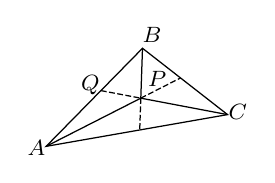
\begin{tikzpicture}[x=.72cm,y=.72cm,line width=.45pt,font=\footnotesize]
 \coordinate (A) at (0,0);
 \coordinate (B) at (1.70,1.73);
 \coordinate (C) at (3.20,.56);
 \coordinate (P) at (1.67,.85);
 \coordinate (Q) at (0.966324,0.983377);
 \coordinate (AC) at (1.650872,0.288903);
 \coordinate (BC) at (2.370863,1.206727);
 \draw (A)--(B)--(C)--cycle;
 \draw (A)--(P) (B)--(P) (P)--(C);
 \draw[dash pattern=on 2.1pt off .9pt] (Q)--(P) (P)--(BC) (P)--(AC);
 \node[inner sep=0pt] at (-.17,-.02) {\(A\)};
 \node[inner sep=0pt] at (1.87,1.96) {\(B\)};
 \node[inner sep=0pt] at (3.38,.60) {\(C\)};
 \node[inner sep=0pt] at (1.96,1.19) {\(P\)};
 \node[inner sep=0pt] at (.78,1.08) {\(Q\)};
\end{tikzpicture}\par}
Since
\[
 Q(AB)=A(BQ)+B(AQ)
\]
\noindent [where \((AB)\) denotes the line segment \(AB\), and so on, it follows that]
\[
 Q(ABC)=A(BQC)+B(AQC)
\]
\noindent [and
\[
 Q(ABP)=A(BQP)+B(AQP);
\]
\noindent hence
\[
 Q(APBC)=A(BPC)+B(APC).
\]
Since, moreover,]
\[
 P(CQ)=Q(PC)+C(PQ)
\]
\noindent [one also has
\[
 P(ABC)=Q(APBC)+C(APB),
\]
\noindent from which the relation first stated follows].\par
}

% Printed 224; principal PDF 231; Google PDF 235.
\par\clearpage
\noindent\makebox[0pt][l]{\fontsize{13}{16}\selectfont 224}\hfill{\small\textbf{POSTHUMOUS PAPERS.}}\hfill\null\par\medskip

\noindent
\begin{tabular}{@{}l@{\enspace}p{.65\linewidth}@{}}
 \(g,g',g''\) \makebox[11em][s]{. . . . . . . . . . . . . . .}&weights [of the corrections]\\
 \(A+\alpha,A'+\alpha',A''+\alpha''\) . . .&azimuths calculated from an approximate position\\
 \(r,r',r''\) \makebox[11.5em][s]{. . . . . . . . . . . . . . . .}&distances [according to the approximate position of the point \(P^0\)].
\end{tabular}

Put
\[
 r\sin(A''-A')=l,\qquad
 r'\sin(A-A'')=l',\qquad
 r''\sin(A'-A)=l'';
\]
\[
 \frac{l\alpha+l'\alpha'+l''\alpha''}
 {\frac{ll}{g}+\frac{l'l'}{g'}+\frac{l''l''}{g''}}=k.
\]

Then the corrected azimuths are:
\[
\begin{aligned}
 {[}A+\delta A={}]&\,A+\frac{lk}{g}\\
 {[}A'+\delta A'={}]&\,A'+\frac{l'k}{g'}\\
 {[}A''+\delta A''={}]&\,A''+\frac{l''k}{g''}.
\end{aligned}
\]

\medskip
{\centering
[3.]\par\smallskip
Adjustment of Three Intersections.\par}
\[
\begin{array}{@{}l@{\;}l@{}}
 a+ib,a'+ib',a''+ib''&\text{the observation stations}\\
 t,t',t''\,.\,.\,.\,.\,.\,.\,.\,.\,.\,.\,.\,.\,.\,.&\text{the three measured azimuths}\\
 \mathrm{d}t,\mathrm{d}t',\mathrm{d}t''\,.\,.\,.\,.\,.\,.\,.\,.\,.\,.\,.&\text{their corrections}\\
 \theta,\theta',\theta''\,.\,.\,.\,.\,.\,.\,.\,.\,.\,.\,.\,.&\text{their tangents}\\
 x+iy\,.\,.\,.\,.\,.\,.\,.\,.\,.\,.\,.\,.\,.\,.&\text{the position to be determined}\\
 X\,.\,.\,.\,.\,.\,.\,.\,.\,.\,.\,.\,.\,.\,.\,.\,.\,.&\text{approximate value of }x\\
 &x=X+\xi.
\end{array}
\]
{\centering Formulas.\par}
\[
\begin{array}{@{}l@{\qquad}c@{}}
 1)&
 \GaussOldenburgLeftBrace{\begin{aligned}
 Y&=b+\theta(X-a)\\
 Y'&=b'+\theta'(X-a')\\
 Y''&=b''+\theta''(X-a'')
 \end{aligned}}\\[3pt]
 2)&r=\dfrac{X-a}{\cos t},\qquad r'=\dfrac{X-a'}{\cos t'},\qquad r''=\dfrac{X-a''}{\cos t''}\\[3pt]
 3)&l=r\sin(t''-t'),\qquad l'=r'\sin(t-t''),\qquad l''=r''\sin(t'-t)
\end{array}
\]

% Printed 225; principal PDF 232; Google PDF 236.
\par\clearpage
\noindent\null\hfill{\small\textbf{TRIGONOMETRIC POINT DETERMINATION.}}\hfill\makebox[0pt][r]{\fontsize{13}{16}\selectfont 225}\par\medskip

\[
\begin{array}{@{}l@{\qquad}c@{}}
 4)&
 \lambda=\dfrac{mlr}{\cos t},\qquad
 \lambda'=\dfrac{ml'r'}{\cos t'},\qquad
 \lambda''=\dfrac{ml''r''}{\cos t''}.
\end{array}
\]

\(m\) is a quantity chosen at will. It is most convenient to choose it so that the smallest of the three numbers \(\lambda,\lambda',\lambda''\) becomes \(1\).
\[
\begin{array}{@{}l@{\qquad}c@{}}
 5)&
 \GaussOldenburgLeftBrace{\begin{aligned}
 y&=Y+\theta\xi+\lambda\varphi\\
 y&=Y'+\theta'\xi+\lambda'\varphi\\
 y&=Y''+\theta''\xi+\lambda''\varphi
 \end{aligned}}
\end{array}
\]
\noindent [are] the equations whose combination determines \(y,\xi,\varphi\).
\[
\begin{array}{@{}l@{\qquad}c@{}}
 6)&\mu=206265m\varphi\\
 7)&\mathrm{d}t=\mu l,\qquad
 \mathrm{d}t'=\mu l',\qquad
 \mathrm{d}t''=\mu l''.
\end{array}
\]

\noindent [The weights of the observations are assumed equal here.]

The same formulas can be used,\kern.45mm\raisebox{.08ex}{\rule{.70mm}{.18mm}} starting from an approximate value of \(y\). Then, apart from the obvious interchanges of \(a\) and \(b\) and of \(X\) and \(Y\), [\(\xi\) and \(\eta\),] \(x\) and \(y\), one need only replace the tangents and cosines of \(t,t',t''\) with their cotangents and sines, and \(\mu\) must be set \(=-206265m\varphi\).

\medskip
{\centering Example for Case 2.\quad (Reduction to the plane already applied)\par}
\[
\begin{array}{@{}l@{\quad}r@{\quad}r@{\quad}r@{\;}r@{\;}l@{}}
 &\multicolumn{1}{c}{[\,a}&\multicolumn{1}{c}{b}
 &\multicolumn{3}{c@{}}{t\,]}\\
 \text{Hamburg}&-224765{,}616\,\mathrm{m}&-2368{,}668\,\mathrm{m}&84^\circ&44'&59''{,}228\\
 \text{Horneburg}&-220411{,}663&+23705{,}056&248&7&57{,}643\\
 \text{Stade}&-230811{,}734&+30884{,}678&300&11&46{,}416\\[3pt]
 \text{York}&&Y=+17377{,}200&&&
\end{array}
\]
\[
\resizebox{\linewidth}{!}{\(\begin{array}{@{}l@{\;}l@{\quad}r@{\;}l@{\quad}r@{\;}l@{}}
 \theta[=\operatorname{cotang}t]\,.&8{,}963\,2724&&9{,}603\,5071&&9{,}764\,8676_{n}\\
 Y-b\,.\,.\,.\,.\,.\,.&4{,}295\,4762&&3{,}801\,2566_{n}&&4{,}130\,5743_{n}\\
 \sin t\,.\,.\,.\,.\,.\,.\,.\,.&9{,}998\,1741&&9{,}967\,5708_{n}&&9{,}936\,6685_{n}\\
 r\,.\,.\,.\,.\,.\,.\,.\,.\,.\,.&4{,}297\,3021&&3{,}833\,6858&&4{,}193\,9058\\
 \sin(t''-t')\,.\,.\,.&9{,}896\,91&\sin(t-t'')\,.\,.\,.&9{,}763\,38&\sin(t'-t)\,.\,.\,.&9{,}456\,33\\
 r:\sin t\,.\,.\,.\,.\,.\,.&4{,}299\,1280&&3{,}866\,1150_{n}&&4{,}257\,2373_{n}\\
 l\,.\,.\,.\,.\,.\,.\,.\,.\,.\,.\,.&4{,}194\,21&&3{,}597\,07&&3{,}650\,24\\
 lr:\sin t\,.\,.\,.\,.\,.&8{,}493\,34&&7{,}463\,18_{n}&&7{,}907\,48_{n}\\
 m\,.\,.\,.\,.\,.\,.\,.\,.\,.\,.&2{,}536\,82_{n}&&2{,}536\,82_{n}&&2{,}536\,82_{n}
\end{array}\)}
\]
\noindent{\small IX.}\hfill{\small 29}\hspace*{.12\linewidth}\par

% Printed 226; principal PDF 233; Google PDF 237.
\par\clearpage
\noindent\makebox[0pt][l]{\fontsize{13}{16}\selectfont 226}\hfill{\small\textbf{POSTHUMOUS PAPERS.}}\hfill\null\par\medskip

\[
\begin{array}{@{}r@{\;}r@{\quad}r@{\quad}r@{}}
 a=&-224765{,}616&-220411{,}663&-230811{,}734\\
 {[}\theta(Y-b)]=&+1814{,}465&-2539{,}591&+7860{,}351\\
 \hline
 X=&-222951{,}151&-222951{,}254&-222951{,}383\\
 \theta\eta=&+0{,}09189\eta&+0{,}40134\eta&-0{,}58193\eta\\
 \lambda\varphi=&-10{,}7192\varphi&+1{,}00000\varphi&+2{,}7816\varphi.
\end{array}
\]

[Solving the equations
\[
\begin{aligned}
 x&=X+\theta\eta+\lambda\varphi\\
 x&=X'+\theta'\eta+\lambda'\varphi\\
 x&=X''+\theta''\eta+\lambda''\varphi
\end{aligned}
\]
\noindent gives:]
\[
\begin{array}{@{}r@{\quad}l@{\quad}r@{}}
 \eta=-0{,}110,&\varphi=+0{,}01169,&x=-222951{,}286\,\mathrm{m},\\
 &\varphi\,.\,.\,.\quad 8{,}06795&y=Y+\eta=+17377{,}090\quad .\\
 \multicolumn{2}{c}{-206265m\,.\,.\,.\quad 7{,}85125}&
\end{array}
\]
\[
 \mathrm{d}t=+1''{,}298,\qquad
 \mathrm{d}t'=+0''{,}328,\qquad
 \mathrm{d}t''=+0''{,}371.
\]

One can also modify the method above by setting
\[
 l=\frac{r}{\cos t}(\theta''-\theta'),\qquad
 l'=\frac{r'}{\cos t'}(\theta-\theta''),\qquad
 l''=\frac{r''}{\cos t''}(\theta'-\theta)
\]
\noindent which saves at least one more logarithm.

\bigskip
{\centering
[4.]\par\smallskip
[On the Adjustment of Three Intersections.]\par}
In general, [let the error equations be]
\[
\begin{aligned}
 ax+by+m&=e\\
 a'x+b'y+m'&=e'\\
 a''x+b''y+m''&=e''.
\end{aligned}
\]
\noindent \(a,b,m,a'\), etc., given; \(x,y\) sought such that
\[
 ee+e'e'+e''e''=\Sigma
\]
\noindent is a minimum.

Put

% Printed 227; principal PDF 234; Google PDF 238.
\par\clearpage
\noindent\null\hfill{\small\textbf{TRIGONOMETRIC POINT DETERMINATION.}}\hfill\makebox[0pt][r]{\fontsize{13}{16}\selectfont 227}\par\medskip

\[
\begin{array}{@{}r@{\;=\;}l@{\qquad}r@{\;=\;}l@{}}
 a&b\theta&m&bn\\
 a'&b'\theta'&m'&b'n'\\
 a''&b''\theta''&m''&b''n'';
\end{array}
\]
\[
 (n-N)(\theta''-\theta')+(n'-N)(\theta-\theta'')+
 (n''-N)(\theta'-\theta)=h,
\]
{\centering \(N\) an arbitrary quantity;\par}
\[
 \frac{\theta''-\theta'}{b}=f,\qquad
 \frac{\theta-\theta''}{b'}=f',\qquad
 \frac{\theta'-\theta}{b''}=f'',
\]
\noindent [then the condition equation follows from the error equations:
\[
 fe+f'e'+f''e''=h].
\]

Then we have [when \(\Sigma\) is minimized subject to this condition:]
\[
\begin{array}{@{}l@{\qquad}c@{}}
 1)&\begin{gathered}
 e=fg,\qquad e'=f'g,\qquad e''=f''g\\
 g=\frac{h}{ff+f'f'+f''f''}
 \end{gathered}
\end{array}
\]
\noindent and
\[
 \Sigma=gh;
\]
\noindent [furthermore, the error equations give:]
\[
\begin{array}{@{}l@{\qquad}c@{}}
 2)&\begin{aligned}
 (\theta''-\theta')x+(n''-n')&=\left(\frac{f''}{b''}-\frac{f'}{b'}\right)g\\
 (\theta-\theta'')x+(n-n'')&=\left(\frac{f}{b}-\frac{f''}{b''}\right)g\\
 (\theta'-\theta)x+(n'-n)&=\left(\frac{f'}{b'}-\frac{f}{b}\right)g.
 \end{aligned}
\end{array}
\]

\(x\) is determined from one of these equations.\\
\hspace*{\parindent}Finally, \(y\) is determined from one of the following:
\[
\begin{array}{@{}l@{\qquad}c@{}}
 3)&\begin{aligned}
 \theta x+y+n&=\frac{e}{b}=\frac{f}{b}g\\
 \theta'x+y+n'&=\frac{e'}{b'}=\frac{f'}{b'}g\\
 \theta''x+y+n''&=\frac{e''}{b''}=\frac{f''}{b''}g.
 \end{aligned}
\end{array}
\]

\medskip
The rules for the adjustment [of three intersections] can [therefore] also be stated as follows, [since, as \(y-b=(x-a)\operatorname{tang}(t+\mathrm{d}t)\) shows, the error equations here have the form
\[
 Y+\eta-b=(X+\xi-a)\left(\operatorname{tang}t+\frac{\mathrm{d}t}{206265\cos t^2}\right),
\]
\noindent\hfill{\small 29\textsuperscript{*}}\hspace*{.12\linewidth}\par

% Printed 228; principal PDF 235; Google PDF 239.
\par\clearpage
\noindent\makebox[0pt][l]{\fontsize{13}{16}\selectfont 228}\hfill{\small\textbf{POSTHUMOUS PAPERS.}}\hfill\null\par\medskip

\noindent or, putting \(\operatorname{tang}t=\theta\),
\[
 \frac{\mathrm{d}t}{206265}=\frac{\cos t^2}{X-a}
 \{-\theta\xi+y-(b+\theta(X-a))\} :]
\]
\[
\begin{array}{@{}c@{\qquad}r@{\qquad}l@{}}
 \ast&1)&Y=b+\theta(X-a)\\[2pt]
 \ast&2)&\rho=\dfrac{X-a}{\cos t^2}\\[4pt]
 \ast&3)&f=\rho(\theta''-\theta')\\[2pt]
 \ast&4)&\nu=\rho f\\[2pt]
 &5)&-h=(\theta''-\theta')(Y-N)+(\theta-\theta'')(Y'-N)+(\theta'-\theta)(Y''-N)\\[2pt]
 &6)&g=\dfrac{h}{ff+f'f'+f''f''}\\[4pt]
 \ast&7)&\mathfrak{Y}=Y+\nu g\\[2pt]
 &8)&y=\mathfrak{Y}+\theta\xi=\mathfrak{Y}'+\theta'\xi=\mathfrak{Y}''+\theta''\xi\\[2pt]
 \ast&9)&\mathrm{d}t=206265fg\\[2pt]
 &10)&\mathrm{d}t^2+\mathrm{d}t^{\prime 2}+\mathrm{d}t^{\prime\prime 2}=206265^2gh.
\end{array}
\]

Each of the formulas 1), 2), 3), 4), 7), 9) marked with \(\ast\) applies in all three cases. In formula 5), \(N\) is arbitrary. One takes one of the quantities \(Y,Y',Y''\) for it.

\(\xi\) and \(y\) are determined from two of the equations in 8).

\bigskip
{\centering
[5.]\par\smallskip
[Determination of a Secondary Point (Schessel) from Observations at Primary Triangulation Stations (Litberg, Wilsede, Bottel, Bullerberg and Brüttendorf).]\par}
\medskip
[Let \(x,y\) be approximate values of the coordinates of the point to be determined, \(a_i,b_i\) the coordinates of the fixed points, and \(T_i\) the azimuths at these points reduced to the plane. If one puts
\[
 x-a_i=r_i\cos t_i,\qquad y-b_i=r_i\sin t_i
\]
\noindent and
\[
 -206265\,.\,\frac{y-b_i}{r_ir_i}=\alpha_i,\qquad
 206265\,.\,\frac{x-a_i}{r_ir_i}=\beta_i
\]
\[
 t_i-T_i=n_i,
\]

% Printed 229; principal PDF 236; Google PDF 240.
\par\clearpage
\noindent\null\hfill{\small\textbf{TRIGONOMETRIC POINT DETERMINATION.}}\hfill\makebox[0pt][r]{\fontsize{13}{16}\selectfont 229}\par\medskip

\noindent then, if \(\mathrm{d}x,\mathrm{d}y\) are the corrections to the approximate values \(x,y\), the error equations have the form:
\[
 v_i=n_i+\alpha_i\mathrm{d}x+\beta_i\mathrm{d}y.
\]
If \(p_i\) is the corresponding weight, the normal equations are therefore:
\[
\begin{aligned}
 {[}p\alpha\alpha]\mathrm{d}x+[p\alpha\beta]\mathrm{d}y+[p\alpha n]&=0\\
 {[}p\alpha\beta]\mathrm{d}x+[p\beta\beta]\mathrm{d}y+[p\beta n]&=0.]
\end{aligned}
\]
\[
\resizebox{\linewidth}{!}{\(\begin{array}{@{}r@{\;}l@{\quad}r@{\quad}r@{\quad}c@{\quad}c@{\quad}l@{}}
 [\,i&&\multicolumn{1}{c}{a_i}&\multicolumn{1}{c}{b_i}&
 \substack{\text{Observed}\\\text{azimuths}}&
 \substack{\text{Reduction}\\\text{to the plane}}&T_i\,]\\
 1&\text{Litberg}&-206866{,}630\,\mathrm{m}&+21895{,}743\,\mathrm{m}
 &20^\circ\,14'\,5''{,}596&-1''{,}522&[\,4''{,}074\\
 2&\text{Wilsede}&-182381{,}889&+210{,}307&90\quad34\quad52{,}1&+0{,}008&\phantom{[\,}52{,}108\\
 3&\text{Bottel}&-168158{,}341&+44014{,}670&222\quad15\quad49{,}801&+1{,}457&\phantom{[\,}51{,}258\\
 4&\text{Bullerberg}&-181819{,}664&+35400{,}829&259\quad15\quad12{,}587&+0{,}075&\phantom{[\,}12{,}662\\
 5&\text{Brüttendorf}&-193340{,}040&+45266{,}609&306\quad22\quad9{,}726&-1{,}090&\phantom{[\,}8{,}636]\\
 \cline{2-4}
 \multicolumn{2}{@{}l}{\text{Schessel:}}&x=-182691{,}501&y=+30807{,}073&&&
\end{array}\)}
\]
\[
\resizebox{\linewidth}{!}{\(\begin{array}{@{}l@{\;}l@{\quad}l@{\quad}l@{\quad}l@{\quad}l@{}}
 &\multicolumn{1}{c}{\text{Litberg}}
 &\multicolumn{1}{c}{\text{Wilsede}}
 &\multicolumn{1}{c}{\text{Bottel}}
 &\multicolumn{1}{c}{\text{Bullerberg}}
 &\multicolumn{1}{c@{}}{\text{Brüttendorf}}\\
 {[}y-b_i\,.\,.\,.\,.\,.\,.&3{,}949\,9425&4{,}485\,6742&4{,}120\,8238_{n}&3{,}662\,1679_{n}&4{,}160\,1544_{n}\\
 x-a_i\,.\,.\,.\,.\,.\,.&4{,}383\,3688&2{,}490\,8178_{n}&4{,}162\,3601_{n}&2{,}940\,4353_{n}&4{,}027\,2900\\
 \cos t_i\,.\,.\,.\,.\,.\,.\,.&9{,}972\,3342&&9{,}869\,2616_{n}&&\\
 \sin t_i\,.\,.\,.\,.\,.\,.\,.&&9{,}999\,9778&&9{,}992\,3161_{n}&9{,}905\,9100_{n}\\
 r_i\,.\,.\,.\,.\,.\,.\,.\,.\,.&4{,}411\,0346&4{,}485\,6964&4{,}293\,0985&3{,}669\,8518&4{,}254\,2444\\
 r_ir_i\,.\,.\,.\,.\,.\,.\,.\,.&8{,}822\,0692&8{,}971\,3928&8{,}586\,1970&7{,}339\,7036&8{,}508\,4888\\
 1:206265\,.\,.&4{,}685\,5749&4{,}685\,5749&4{,}685\,5749&4{,}685\,5749&4{,}685\,5749\\
 r_ir_i:206265\,.&3{,}507\,6441&3{,}656\,9677&3{,}271\,7719&2{,}025\,2785&3{,}194\,0637\\
 \alpha_i\,.\,.\,.\,.\,.\,.\,.\,.\,.&0{,}442\,30_{n}&0{,}828\,71_{n}&0{,}849\,05&1{,}636\,89&0{,}966\,09\\
 \beta_i\,.\,.\,.\,.\,.\,.\,.\,.]&0{,}875\,72&8{,}833\,85_{n}&0{,}890\,59_{n}&0{,}915\,16_{n}&0{,}833\,23
\\[2pt]
 \multicolumn{6}{@{}l@{}}{t_i=20^\circ\,14'\,4''{,}823,\quad
 90^\circ\,34'\,47''{,}151,\quad222^\circ\,15'\,51''{,}324,\quad
 259^\circ\,15'\,13''{,}643,\quad306^\circ\,22'\,9''{,}500}\\
 \hline
 [\,n_i=&+0{,}749&-4{,}957&+0{,}066&+0{,}981&+0{,}864\\
 \alpha_i\mathrm{d}x=&-2{,}769\,\mathrm{d}x&-6{,}741\,\mathrm{d}x&+7{,}064\,\mathrm{d}x&+43{,}340\,\mathrm{d}x&+9{,}249\,\mathrm{d}x\\
 \beta_i\mathrm{d}y=]&+7{,}511\,\mathrm{d}y&-0{,}068\,\mathrm{d}y&-7{,}773\,\mathrm{d}y&-8{,}225\,\mathrm{d}y&+6{,}811\,\mathrm{d}y.
\end{array}\)}
\]

[The error equation for Wilsede was given the weight \(p_2=\tfrac1{25}\), and the remaining error equations were given equal weights, \(p_i=1\).]

% Printed 230; principal PDF 237; Google PDF 241.
\par\clearpage
\noindent\makebox[0pt][l]{\fontsize{13}{16}\selectfont 230}\hfill{\small\textbf{POSTHUMOUS PAPERS.}}\hfill\null\par\medskip

\[
\resizebox{\linewidth}{!}{\(\begin{array}{@{}r@{\;}r@{\;}r@{\quad}r@{\;}r@{\;}r@{\quad}l@{\quad}l@{}}
 p\alpha\alpha&p\alpha\beta&p\alpha n&p\beta\beta&p\beta n&pnn&&\\[1pt]
 7{,}666&-20{,}798&-2{,}074&56{,}421&+5{,}626&0{,}5610&
 \Bigl[[p\alpha\alpha]\,.\,.\,.\,.\,.\,.\,3{,}30606&\\[5pt]
 1{,}818&+0{,}018&+1{,}337&0{,}000&+0{,}014&0{,}9829&
 [p\alpha\beta]\,.\,.\,.\,.\,.\,.\,2{,}56724_{n}&
 \Biggl[\dfrac{[p\alpha\beta]}{\surd[p\alpha\alpha]}\,.\,.\,.\,.\,.\,.\,0{,}91421_{n}\\[5pt]
 49{,}900&-54{,}909&+0{,}466&60{,}420&-0{,}513&0{,}0044&
 [p\alpha n]\,.\,.\,.\,.\,.\,.\,\underline{1{,}70102}&
 \phantom{\Biggl[}\dfrac{[p\alpha n]}{\surd[p\alpha\alpha]}\,.\,.\,.\,.\,.\Biggr]\,0{,}04799\\[5pt]
 1878{,}360&-356{,}492&+42{,}517&67{,}658&-8{,}069&0{,}9624&
 \surd[p\alpha\alpha]\,.\,.\,.\,.\,1{,}65303&\\[7pt]
 85{,}542&+62{,}997&+7{,}991&46{,}394&+5{,}884&0{,}7465&
 [p\beta\beta.1]\,.\,.\,.\,.\,2{,}21360&\\[4pt]
 \cline{1-6}
 2023{,}286&-369{,}184&+50{,}237&230{,}893&+2{,}942&3{,}2572&&\\[4pt]
 &&&67{,}363&-9{,}166&1{,}2473&
 [p\beta n.1]\,.\,.\,.\,.\,\underline{1{,}08307}&
 \left[\dfrac{[p\beta n.1]}{\surd[p\beta\beta.1]}\,.\,.\,.\right]9{,}97627\\[5pt]
 \cline{4-6}
 &&&163{,}530&+12{,}108&2{,}0099&
 \surd[p\beta\beta.1]\,.\,.\,.\,1{,}10680&\\[4pt]
 \multicolumn{6}{r}{\left[\dfrac{[p\beta n.1]^2}{[p\beta\beta.1]}=\right]\underline{0{,}8965}}&
 \mathrm{d}y\,.\,.\,.\,.\,.\,.\,.\,.\,8{,}86947_{n}&\\[5pt]
 \multicolumn{6}{r}{\bigl[[pvv]=\bigr]1{,}1134}&
 \dfrac{[p\alpha\beta]}{[p\alpha\alpha]}\,.\,.\,.\,.\,.\Biggr]\,\underline{9{,}26118_{n}}&
\end{array}\)}
\]

\noindent
\begin{minipage}[t]{.55\linewidth}
 [The coordinates of \textls[120]{Schessel}\\
 are therefore:
 \[
 \begin{aligned}
  x&=-182691{,}539\,\mathrm{m}\\
  y&=+\phantom{1}30806{,}999\quad .]
 \end{aligned}
 \]
\end{minipage}\hfill
\begin{minipage}[t]{.43\linewidth}
 \[
 \begin{array}{@{}r@{\;}r@{}}
  \Biggl[\dfrac{[p\alpha\beta]}{[p\alpha\alpha]}\mathrm{d}y=&+0{,}01351\\[5pt]
  \dfrac{[p\alpha n]}{[p\alpha\alpha]}=\Biggr]&+0{,}02483\\
  \cline{2-2}
  \mathrm{d}x=&-0{,}038\\
  \mathrm{d}y=&-0{,}074.
 \end{array}
 \]
\end{minipage}\par

[The errors remaining after the adjustment are:]
\[
\begin{array}{@{}r@{\;}r|r|r|r|r@{}}
 [t_i-T_i=&+0{,}749&-4{,}957&+0{,}066&+0{,}981&+0{,}864\\
 \alpha_i\mathrm{d}x=&+0{,}1052&+0{,}2562&-0{,}2684&-1{,}6469&-0{,}3515\\
 \beta_i\mathrm{d}y=&-0{,}5558&+0{,}0050&+0{,}5752&+0{,}6087&-0{,}5040\\
 \hline
 v_i=]&+0{,}298&-4{,}696&+0{,}373&-0{,}057&+0{,}009.
\end{array}
\]

% Printed 231; principal PDF 238; Google PDF 242.
\par\clearpage
\noindent\null\hfill{\small\textbf{TRIGONOMETRIC POINT DETERMINATION.}}\hfill\makebox[0pt][r]{\fontsize{13}{16}\selectfont 231}\par\medskip

\vspace*{3.6\baselineskip}
{\centering
[6.]\par\medskip
{\footnotesize
\begin{tabular}{c}
\hline
Astronomische Nachrichten. Vol. I. No. 6, pp. 81—86. 1823.\\
\hline
\end{tabular}\par}
\medskip
Application of the Calculus of Probabilities to a Problem\\
in Practical Geometry.\par}
\medskip

In accordance with your request, I am sending you the rules for applying the method of least squares to the following problem in practical geometry. Find the position of a point from the horizontal angles measured at it between other points whose positions are known exactly. The subject is quite elementary, and anyone familiar with the spirit of the method of least squares can easily derive the rules for themselves. Yet since the problem is one of the most useful in practical geometry, it may often be taken up by people who are not quite in that position and who will therefore welcome having the formulas.

Let the coordinates of one of the known points be \(a,b\), the former counted positively from north to south and the latter from east to west. Whether the axis of abscissas is a true meridian is immaterial here. Likewise, let \(x,y\) be approximate coordinates of the point to be determined and \(\mathrm{d}x,\mathrm{d}y\) their as yet unknown corrections. Determine \(\varphi\) and \(r\) by the formulas
\[
 \operatorname{tang}\varphi=\frac{b-y}{a-x},\qquad
 r=\frac{a-x}{\cos\varphi}=\frac{b-y}{\sin\varphi},
\]
\noindent choosing \(\varphi\) in the quadrant that makes \(r\) positive, and also put
\[
 \alpha=\frac{206265\,.\,(b-y)}{rr},\qquad
 \beta=-\frac{206265\,.\,(a-x)}{rr}.
\]

Then the azimuth of the first point as seen from the second (taking the direction of the axis of abscissas as \(0\)),
\[
 =\varphi+\alpha\mathrm{d}x+\beta\mathrm{d}y,
\]
\noindent where the last two terms are expressed in arcseconds.
